\documentclass[procedia]{easychair}
\usepackage{url}
\usepackage[flushleft]{threeparttable}
\hyphenation{resour-ces}
\hyphenation{approac-hes}
\hyphenation{har-der}
\hyphenation{spe-cifically}
\makeatletter
\def\@copyrightspace{\relax}
\makeatother

\usepackage{comment}
\excludecomment{TM}
%\setlength{\textwidth}{6.25in}

\title{An Invariant Framework for Conducting Reproducible Computational Science}

% \titlerunning{} has to be set to either the main title or its shorter
% version for the running heads. When processed by
% EasyChair, this command is mandatory: a document without \titlerunning
% will be rejected by EasyChair

\titlerunning{An invariant framework for conducting reproducible computational science}

\author{
	Haiyan Meng\inst{2}
\and Rupa Kommineni\inst{1}
\and Quan Pham\inst{1} \\
\and Robert Gardner\inst{1}
\and Tanu Malik\inst{1}
\and
	Douglas Thain\inst{2}
}
\institute{
	Computation Institute,
	University of Chicago,
	Chicago, Illinois, USA \\
	\email{rupa, quanpt, rwg, tanum@uchicago.edu}
\and
	Department of Computer Science and Engineering,
	University of Notre Dame,
	Notre Dame, Indiana, USA \\
	\email{hmeng, dthain@nd.edu}
}

%  \authorrunning{} has to be set for the shorter version of the authors' names;
% otherwise a warning will be rendered in the running heads. When processed by
% EasyChair, this command is mandatory: a document without \authorrunning
% will be rejected by EasyChair

\authorrunning{Meng et al.}

\begin{document}

\maketitle

\keywords{Preservation framework, reproducible research, virtualization, container}

\begin{abstract}
\it Computational reproducibility depends on being able to isolate necessary and sufficient computational artifacts and preserve them for later re-execution.
Both isolation and preservation of artifacts can be challenging due to the complexity
of existing software and systems and the resulting implicit dependencies, resource distribution, and shifting compatibility of systems as time progresses---all conspiring
to break the reproducibility of an application. Sandboxing is a technique
that has been used extensively in OS environments for isolation of computational artifacts.
Several tools were proposed recently that employ sandboxing as a mechanism to ensure reproducibility.
However, none of these tools preserve the sandboxed application for re-distribution
to a larger scientific community---aspects that are equally crucial for ensuring reproducibility as sandboxing itself.
In this paper, we describe a combined sandboxing and preservation framework, which is efficient, invariant and
practical for large-scale reproducibility. We present case studies of complex high energy
physics applications and show how the framework can be useful for sandboxing, preserving and distributing applications.
We report on the completeness, performance,
and efficiency of the framework, and suggest possible standardization approaches.
\end{abstract}

% A category with the (minimum) three required fields
%\category{H.4}{Information Systems Applications}{Miscellaneous}
%A category including the fourth, optional field follows...
%\category{D.2.8}{Software Engineering}{Metrics}[complexity measures, performance measures]

%\terms{Theory}

\section{Introduction}

Reproducibility is a cornerstone of the scientific method~\cite{borgman2012data}. 
Its ability to advance science underscores its importance---reproducing by verifying and validating a scientific result leads to improved understanding, thus increasing possibilities of reusing or extending the result. 
Ensuring the reproducibility of a scientific result, however, often entails detailed documentation and specification of the involved scientific method. Historically, text and proofs in a publication have achieved this end. 
As computation pervades the sciences and transforms the scientific method, mere text is no longer sufficient. 
In particular, apart from textual descriptions describing the result, a reproducible result must also include several computational artifacts, such as software, data,  environment variables, and the state of computation that are involved in the adopted scientific method \cite{Sole}.  

Virtualization has emerged as a promising way to reproduce computational scientific results. One such approach is to conduct the entire computation relating to a scientific result within a virtual machine image, and then share the resulting image. This way VMIs become an authoritative, encapsulated, and executable record of computations, especially computations whose results are destined for publication and/or re-use; images, like files, can then be shared \cite{Lampoudi}. 
The resulting image, however, may be too big to share or distribute widely. An alternative light-weight form of virtualization is to encapsulate only the application software along with all its necessary dependencies into a self-contained package. The encapsulation is achieved by OS-level sandboxing techniques that interpose application system calls and copy the necessary dependencies (data, libraries, code, etc.) into a package, making it lighter weight than a VMI~\cite{guo2011cde}. Yet, the package is not longer an executable record of the computation and still requires an accompanying operating system for execution. 

While both approaches provide mechanisms for encapsulating the computations associated with a scientific result, neither form of virtualization provides any guarantee that the included pieces of software will indeed reproduce the associated scientific result. In general, in the absence of reproducible policy guidelines, such guarantees can be difficult to provide. Preserving the encapsulated computations in such a way that they are always reproducible will improve upon the guarantees. A preservation mechanism can increase the ease of image or package installation, alter dependencies implicit to computation as software components evolve or become deprecated, and provide mechanisms for documentation that make computations easy to understand.

%Since reproducibility includes documentation, virtualization approaches in their current form only make it easy to capture the computations. Preserving the computations so that they are easy to understand, install, or alter implicit dependencies that are part of computation is not effectively addressed, especially as dependencies and software components evolve or become deprecated. 

The two approaches that address the preservation challenge are as follows: one, the introduction of tools that help document dependencies and provide software attribution within VMIs or packages; and two, the use of software delivery mechanisms such as centralized package management, Linux containers, and the more recent Docker framework. We examined the first approach previously in \cite{SoftProv}. 
In this paper we examine the second approach.  We consider in particular the lightweight virtualization because we believe together with more standardized software delivery mechanisms, the two combined can address the reproducibility challenge for a wide variety of scientific researchers. A package created by those lightweight approaches encapsulates all the necessary dependencies of an application, and can be used to repeat the application through different sandbox mechanisms, including Parrot
%In particular, we consider the light-weight virtualization approaches, because, we believe that a combination of light-weight approaches with more standardized software delivery mechanisms can lead to addressing the reproducibility challenge for a wide variety of scientific researchers.  
%A package created by those light-weight approaches encapsulates all the necessary dependencies of an application, and can be used to repeat the application through different sandbox mechanisms, including Parrot
~\cite{thain2005parrot}, CDE~\cite{Guo}, PTU~\cite{PTU}, chroot, and Docker~\cite{boettiger2015introduction}. 

Of course our solution represents only one way to preserve applications. Broadly, two different approaches to preserve applications have been adopted: force cleanliness or measure the mess. The former forces users to specify the execution environment for an application in a well-organized way. The latter causes end users to construct the environment as desired, and the complexity of the environment is measured in terms of its dependencies. Our objective here is to measure the mess as-is and then preserve it over time.

%We do not claim our solution is the only way to preserve applications. Broadly, there are two different approaches to preserve applications: force cleanliness or measure the mess. The first approach forces users to specify the execution environment for an application in a well organized way. In the latter one end users construct the environment as desired, and the complexity of the environment is measured in terms of its dependencies. 
%Our objective here is to measure the mess as-is and then preserve it over time.

To conduct a thorough examination, we consider real-world complex high energy physics (HEP) applications, independently developed by two groups, that must be reproduced so that the entire HEP community can benefit from the analysis. We describe challenges faced in reproducing the applications, and we consider the extent to which reproducibility requirements can be satisfied with lightweight virtualization approaches and software delivery mechanisms. We propose an invariant framework for computational reproducibility that combines lightweight virtualization with software delivery mechanisms for efficiently capturing, invariantly preserving, and practically deploying applications. We measure the performance overhead of lightweight virtualization and software delivery approaches, and show how the preserved packages can be distributed to allow reproduction and verification.
%To conduct a thorough examination, we consider real-world complex high energy physics (HEP) applications, independently developed by two groups, that must be reproduced so that the entire HEP community can benefit from the analysis. We describe challenges in reproducing the applications, and consider the extent to which reproducibility requirements can be satisfied with light-weight virtualization approaches and software delivery mechanisms. We propose an invariant framework for computational reproducibility that combines light-weight virtualization with software delivery mechanisms for efficiently capturing, invariantly preserving and practically deploying applications.
%We measure the performance overhead of  light-weight virtualization and software delivery approaches, and show the preserved packages can be distributed to allow reproduction and verification.


\section{High Energy Physics Applications}

We study applications taken from two experiments of the CERN Large Hadron Collider, namely the ATLAS experiment and the CMS experiment. 
One of the applications of the ATLAS experiment is the \emph{Athena} application, which is a general purpose processing framework including algorithms
for event reconstruction and data reduction \cite{calafiura2005athena}. The CMS experiment is conducted through an application termed  \emph{TauRoast}, which searches for specific 
cases where the Higgs boson decays to two tau leptons~\cite{chatrchyan2013search}. In LHC, the ATLAS and CMS experiments are distinct, 
developed independently by two entirely separate physics communities. Consequently, their applications  
have very different software distribution and data management frameworks, making it interesting to examine if common reproducibility frameworks and 
tools work across the two communities. 

Code and data in \emph{TauRoast} is available through five different networked filesystems, namely an HDFS cluster for data files, 
some configuration files were stored on a CVMFS~\cite{blomer2011cernvm} filesystem, and a variety of software tools were on an NFS, PanFS and AFS systems.
In addition, code may exist in version control systems such as Git, CVS, and CMS Software Distribution (CMSSW). %~\cite{cms2006cms}. 
\begin{wrapfigure}{r}{0.4\textwidth}
\small
\centering
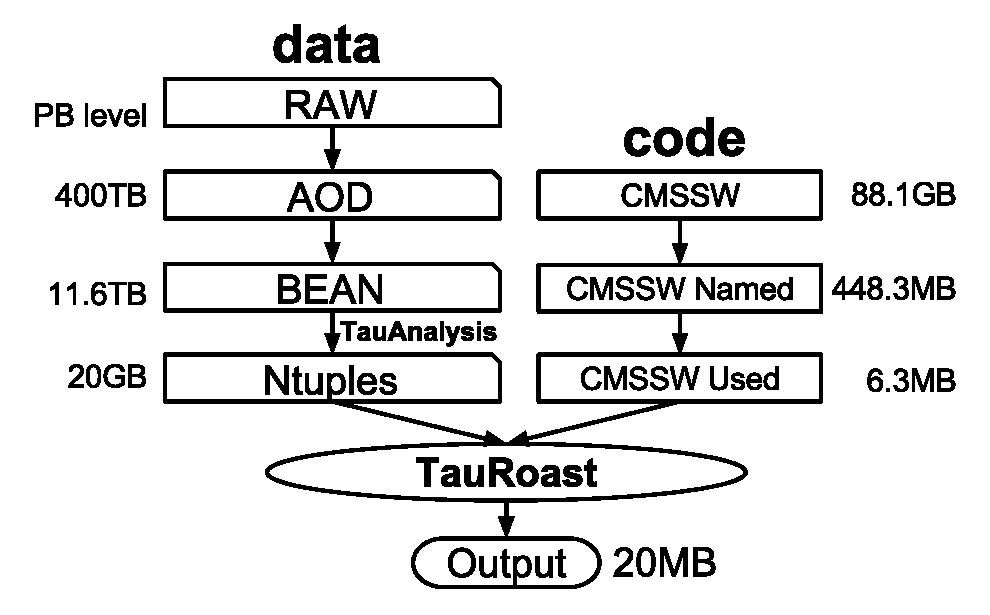
\includegraphics[width=.4\textwidth]{data-code-size.eps}
\caption{Inputs to Tau Roast}
\label{fig:data-code-size}
\end{wrapfigure}
Data that is input to \emph{TauRoast} is obtained by reducing it through a pipeline, as shown in Figure \ref{fig:data-code-size}. Consequently, the real input data may 
vary depending upon the science question being researched. Similarly the software may name many possible components but the used components are
smaller than the named ones. 

In \emph{Athena} data is obtained through an external Dropbox-like system called the FaxBox, but does not go through any reduction steps. Code is obtained through 
CVMFS, which provides the analysis routines. However, depending upon the input data code and the configuration that will be invoked changes. 
Thus in \emph{Athena} the used code and configuration are dynamic depending upon input data, where as in \emph{TauRoast} the code and data are static, 
but the amount of data and code to include changes depending on the involved science. 


\section{Challenges in Reproducing HEP Applications}

The application specifications of \emph{TauRoast} and \emph{Athena} were provided to us from the CMS and ATLAS Collaborations respectively in the form of 
email describing in prose how to obtain the source, build the program, and run it correctly on a specific platform type available at our home institutions.  There were no explicit guarantees that it would run on alternative platforms.  This minimal level of documentation about software is routine in the scientific world. 
Below we describe the challenges faced when capturing application details in reproducible form and then preserving them for subsequent reuse.

\begin{itemize}

\item {\bf Identifying all dependencies.}  Due to the distributed, collaborative nature of HEP software development, these applications depend on a large number of external and local software components.
External dependencies are often explicitly stated, such as when the application makes connections to Github resources or CVS servers for downloading source files. 
When the application has initiated execution then implicit network connections may be present that require identification of dependencies on all machines where execution takes place. 
Implicit local dependencies can arise as a result of mounted filesystems. In \emph{TauRoast}, the application data and code is distributed on five networked filesystems, and in \emph{Athena} on two networked filesystems. 
Since these filesystems appear local to the application machine, it is important to check and capture mounted filesystems and their respective mount points. 

\item {\bf Configuration Complexity.} In order to correctly reproduce an application requires that run-time configurations and consistency checks on the available software are effectively captured and preserved. 
For CMS,  the {\tt scram} software management tool is used to locate
the appropriate version of software,  set environment variables such as the PATH, run any
tool-specific configurations, and do the same for all software on which it depends. A reproducible framework must capture the work of such software management tools so that the framework can conduct similar checks on a new machine. 

\item {\bf High Selectivity.}  
Although the total size of the resources accessed by HEP programs is very large, the size of the data and software actually used are typically much smaller. The script will often name an entire repository or data source, but the program needs only a handful of items from that source. For example, the data may be stored on an HDFS filesystem with 11.6TB of data, but the program may consume only 18GB. Thus there is a size tradeoff in terms of capturing dependencies mentioned in the program and dependencies actually used in the program. A reproducible framework must include robust rules about not including superfluous dependencies, but including unused dependencies that may potentially see much use during program execution.

\item {\bf Rapid Changes in Dependencies.}  
Over the course of three months between collecting the initial email, analyzing the programs, and writing this paper, the computing environment saw continuous change. The CMSSW software distribution released a new version, the target execution environment was upgraded to a new operating system, and the application switched from CVS to Git for obtaining the software. For Athena, the computing environment has the potential for daily change since upgrades to the software framework occur on a nightly basis. While the users of this software seem accustomed to constant change, which is appropriate during algorithm development, any new technique for preservation that may rely on an external service (every one that may appear highly stable) will require caution to choose the actual releases used during the time of publication.

\item {\bf Dependencies for Reproducible Execution.} Capturing the necessary and sufficient dependencies that are part of an application is sufficient for repeatability, but possibly for not reproducibility.
Repeatability implies that if a result depends on running program X, we must be able to run exactly X again. In reproducibility the goal is rarely limited to running
\emph{precisely} what a predecessor did. Often, the objective is to
change a parameter or a data input in order to see how the result is affected. To that end, the preservation system must capture enough of the surrounding
material in order to permit modifications to succeed. 
Further, a better understanding of how end users will consume preserved software will help to shape how
software should be preserved.
\end{itemize}


\section{The Invariant Framework}

Given the many challenges of reproducing HEP applications, we now describe an invariant framework, which if present within large collaborations, can enable application developers to share their 
application with other researchers, and for other researchers to reproduce the shared application. 
To satisfy invariance, the framework must include mechanisms for:

\begin{itemize}

\item {\bf Capturing Dependencies and Configurations:} Capturing tools must record dependencies that are used by the program, including hardware, OS, kernels, static and dynamic dependencies, local and networked dependencies, source codes and data files. Stateful interactions with commercial software, such as proprietary databases and which cannot be captured due to licensing agreements must be persisted so that they can replayed later without the presence of the commercial software.  In effect, a captured application should behave exactly the same way as the application developer intended it to be. 
% In audit phase, PTU captures the execution of the application into a package. The resulting package contains the source code, its dependencies (system files, and files on network such as from CernVM-FS) and the data consumed and written by the application.

\item{\bf Preservation of Captured Entities:} By preservation we imply appropriate mechanisms for (a) documentation of the application development, and (b) automation of any task that becomes inevitably 
necessary for repeating the application in exactly the same way as the developer executed it. 
 
Documentation and specification during application development can be an onerous one. The preservation framework must make programming tools available that 
focus less on documentation, but script, integrate and execute the dependencies so that they are resolved as part of documentation. 
Automation can extend to various tasks that are necessary for ensuring repeatability such as building software, provisioning of hardware, 
validation of software against security fixes, new features, and even monitoring the reproducibility state of a preserved application, i.e., its source code, dependencies, environment, and platform.
Automated builds and provisioning and continuous integration service can significantly lower the barrier to run the application in a new environment. 

In spite of the preservation mechanisms, the application software may not run as intended. For a reproducer's understanding, it may also be useful to include 
a \emph{logical preservation unit} (PLU) that consists of a minimal execution of the software using a small, test data sample, and with specified outputs.
The provenance of this PLU must be captured so that the reproducer can make comparison with future reproduction-validation runs. 

\item {\bf Distribution of Preserved Packages:} A captured and preserved application must be persistently stored and distributed through a repository. We imagine these repositories to be themselves preserved, and linked with a digital library. Metadata and flexible annotation should be part of this repository for curation over time. 

\end{itemize}


%\section{Evolving the Artifact}
%
%\begin{figure*}[t]
%\centering
%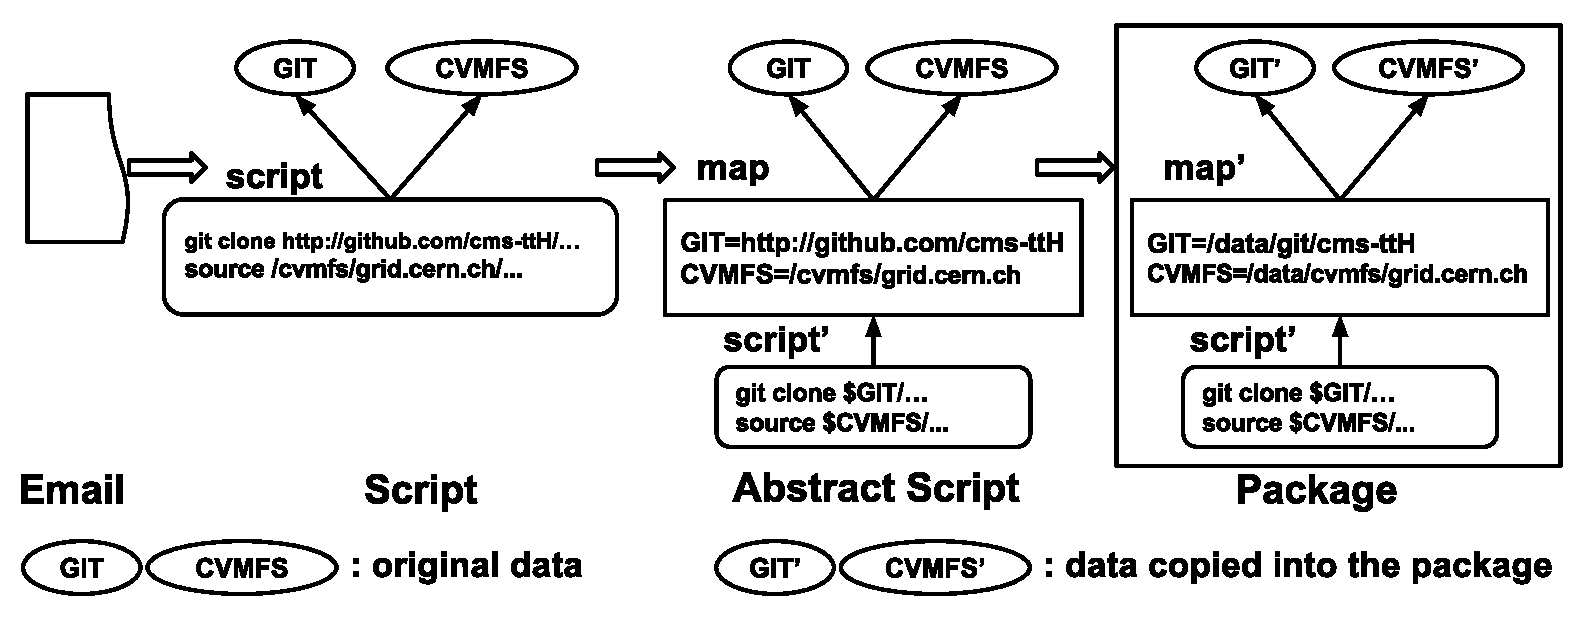
\includegraphics[width=.8\textwidth]{version-evolution.eps}
%\caption{Version Evolution}
%\label{fig:version-evolution}
%\end{figure*}
%
%It is clear that the artifact, as provided, is not in a suitable form
%for preservation.  While it might be technically possible to automatically
%capture the entire virtual machine and all of the connected filesystems,
%it would require 166.8TB of storage, which would be prohibitively expensive
%for capturing this one application alone.  Further, if multiple
%similar applications are preserved, we would miss the opportunity to identify
%common dependencies and store them once for multiple artifacts.
%A more structured approach to dependency management is needed.
%
%Figure~\ref{fig:version-evolution} shows how we have evolved this artifact
%through several stages which make it more suitable for preservation.
%In each step of evolution, we make the dependencies of the artifact
%more explicit and available for analysis and automated processing.
%As noted in the previous section, the original author provided us with
%prose instructions by email which we translated into an
%executable script.  The executable script has embedded in it
%a number of external identifiers such as URLs pointing to repositories
%and paths to networked filesystems.  As a general programming practice,
%embedding such constants into the middle of a program is unwise, and so
%we extract all of those identifiers and place them \emph{outside} the
%script in a \emph{dependency map} or just \emph{map} for short.
%The dependency map lists all of the external dependencies of the application, indicating
%the type, how they are accessed, and where they are currently located.
%The resulting script then simply refers to abstract file locations such
%as \verb$GIT$ and \verb$CVMFS$, while the map file indicates where they
%are currently located. If properly constructed, the script should not refer to any external
%resource unless it is indicated in the dependency map.  We call this idealized
%artifact an \emph{abstract script}.
%
%By extracting the dependencies into the dependency map,
%we introduce great freedom for the curator to move, transform, and otherwise
%manipulate the dependencies of the artifact without damaging the artifact itself.
%A Figure~\ref{fig:version-evolution} shows, it is straightforward for an
%automated tool to examine
%all of the dependencies in the map, download those that are missing,
%and then modify the map to point to the local copies of the dependencies.
%If we group the script, dependency map, and dependencies into a \emph{package},
%we now have a self-contained artifact that can be moved from place to place.
%In some cases, it may be safe to allow the dependency map to refer to 
%trusted remote repositories.  Whether this is advisable is a judgment that
%must be made by the user or the curator, taking into account the long-term
%stability of said repositories.
%
%However, only having the package and the dependency map is not enough. The successful execution of the application on the original machine also relies on the configuration of environment variables.
%We collected the environment variables of the original machine and transformed it into one executable script. If another researcher wants to repeat the application, this executable script will be first executed. 
%The environment variables refer to the dynamic named values defined in the range of one computer, like \verb!$PATH! and \verb!$PYTHONPATH!.
%However, the dependency map refers to the actual storage location of path variables used in one abstract script. For example, the actual storage location of the path variable \verb!CVMFS! 
%is {\tt /data/cvmfs/grid.cern.ch}.
%
%\begin{figure}
%\centering
%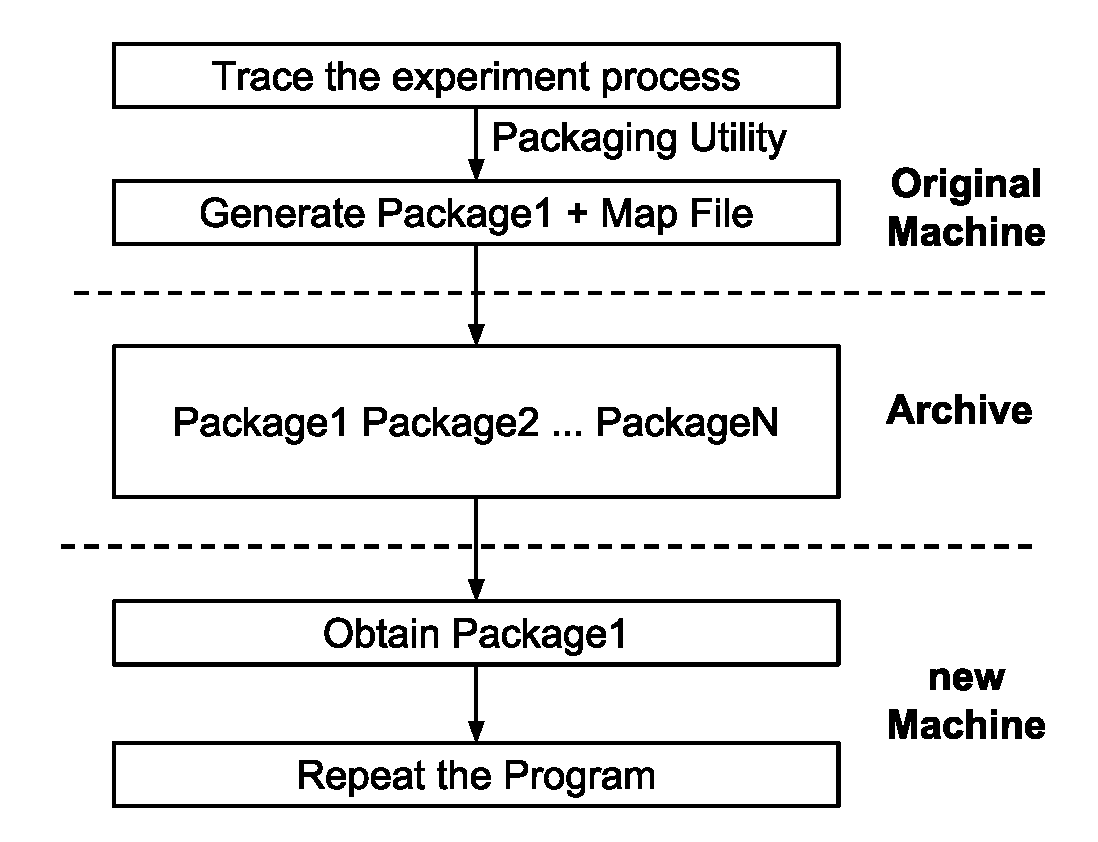
\includegraphics[width=.5\textwidth]{solution3.eps}
%\caption{Relationship of Roles}
%\label{fig:solution3}
%\end{figure}
%
%The relationship of different roles involved in the application preservation and
%reproduction is shown in Figure~\ref{fig:solution3}.  The original author uses the packaging utility to generate the package for one application.
%Then the package, together with
%its map file and description file will be published. When
%another researcher wants to repeat the application, one copy of the package will be downloaded into the new machine and the application can be repeated.
%
%When we try to repeat one application on one new machine, one map file is necessary for the relocation of the data access targets, as
%show in Figure~\ref{fig:version-evolution}. 
%The map file clearly defines the real location of each dependency in the format of dependency variables - the real location of dependency variable {\tt GIT} is \path{/data/git/cms-ttH} and the real location of dependency variable {\tt CVMFS}
%is {\tt /data/cvmfs/grid.cern.ch}.
%The script only refers to the dependency variables defined in the map file.
%This design decouples the application script and the actual data access targets, which minimizes the impact of the evolution of different data dependencies
%and ensures the transparent access.
%The modification of the package only introduces the minimal changes of the map file on the client side.
%
%This basic approach to dependency management is a step in the right direction
%for dependencies that are \emph{explicit} and \emph{external} to the
%user's native execution environment.  However, it leaves two other problems unsolved.
%
%First, the basic approach requires that someone be \emph{aware} of the dependencies,
%whether it be the end user, the system administrator, or the archive curator.
%It seems reasonable to expect the user to be aware of a large dependency mentioned in a top-level script.
%But, oftentimes the dependency is embedded invisibly deep within the software stack,
%or is connected to the machine by the local system administrators.  No single party
%is likely to have complete information about all of the dependencies.
%Second, the basic approach assumes that the entire dependency is actually
%consumed by the artifact.  As we have suggested above (and will show below),
%this sort of program often only consumes a small fraction of what it does declare
%as a dependency.
%
%To address both of these problems, users and curators alike need tools that
%will automatically observe the dependencies of complex applications, to
%facilitate automatic and efficient preservation.
%

\section{Component Tools for Reproducible Research}

We describe some tools that can be used as part of the reproducible framework, and ensure invariance:

\subsection{Capture tools} For capture we focus on automated tools for capturing dependencies (both software and data) instead of manual tools such as makefiles and configuration scripts, since the latter cannot ensure invariance. 
%Parrot

\vspace{5pt}
\noindent {\bf Parrot} Parrot is a virtual filesystem access tool which has been used to attach
existing programs to a variety of remote I/O systems, such as HTTP, FTP, and CVMFS.
It works by trapping an application's system calls through the Linux {\tt ptrace} debugging
interface, and then replacing them with the desired I/O operations. 
To capture dependencies, Parrot records a \emph{namelist} which lists all 
of the files that an application actually accesses. Using the namelist, Parrot creates a \emph{reduced package} which contains
only the files actually used by the application.

Being tightly integrated with I/O systems, the Parrot virtual filesystem is required to be installed for both audit and execution to allow for reproducibility.
In the high energy physics community, Parrot is already used to 
provide access to the CMSSW software distribution via the CVMFS distributed file system.
and is thus invariant for applications like TauRoast. However, unless installed, Parrot cannot ensure invariance for general applications. 

% PTU
\vspace{5pt}
\noindent{\bf PTU} PTU creates a package of an application by recording program binaries, libraries, scripts, data files, and environment variables, etc. It also uses the UNIX \emph{ptrace} system call interposition to identify the code and data used by the running application. PTU was forked from CDE \cite{}, and was thus limited to major Linux kernel versions (e.g. 2.6.x); consequently we have removed that restriction by adapting it for the newly released Linux kernel 3.0 as well as for Mac OS X \cite{}. Thus PTU provides OS invariance and does not require installation and configuration. 

\subsection{Preservation tools}

% Parrot package
\vspace{5pt}
\noindent{\bf Parrot:} In Parrot, the package is preserved based on user option.  
In a {\bf shallow copy}, only individual files in the namelist are copied,
creating only parent directories for each.  Where a directory was listed,
a directory is created and populated with empty files as placeholders
to facilitate a directory listing.  In a {\bf medium copy}, 
individual files are copied as before and directory contents, one level deep are copied. A {\bf deep copy}, which can duplicate all directories recursively,
resulting in TB-sized packages, is not allowed. 

% PTU package
\vspace{5pt}
\noindent{\bf PTU:} Owing to CDE, in PTU, the complete package is preserved, consisting of all code and data files, however deep the data paths are. 
In CDE a binary only captures a single execution path, which is the execution path taken during run-time. If different execution paths need different types of dependencies, some dependencies may be left out. To preserve these dependencies, we have added addition functionality in PTU. In particular, information about other static binaries and required static shared libraries, such as version number, released version of shared libraries, and associated kernel distribution, is preserved using UNIX commands file, ldd, strings, and objdump \cite{}. We also have added a provenance wrapper over CDE \cite{}. This provenance wrapper documents all the dependencies, and provides information about process execution times and memory consumption. It creates a graph of the reference execution providing details about how data was created and transformed as part of the execution. The proevenance description is analgalous to the logically preserved unit. 

Neither the Parrot packages or extended CDE package provide a literate programming environment or a continuous integration environment for changes in software. Thus they are preserved but make break over time as technology changes.
 
 % Docker images
\vspace{5pt}
\noindent{\bf Linux Containers and Docker Images:} Linux Containers provide multiple isolated execution instances on top of the same kernel through OS-level virtualization. Thus they can be used to persist the captured packages into images. Using such containers, Docker now allows to preserve the image in a more user-friendly way. In particular, apart from performing Linux container (LXC) based operating system (OS) level virtualization, docker tools provides portable deployment of containers across platforms, documentation of packages in a scriptable format, and versioning of container images. The image can be preserved along with dockerfiles, which are plain text files with a literate programming environment: the computational part is similar to shell scripts and can help provision similar to other provisioning tools (e.g. Chef, Puppet) or Continuous Integration (CI) platforms (e.g. Travis CI), and the text part is for human consumption and more suited for use with a version management system such as subversion or git, which can track any changes made to the Dockerfile. Thus dockerfiles can be used to preserve the namelist of Parrot packages and provenance description in PTU. 
Docker is integrated with a continuous build environment which will check and validate the version of the software being used, and use a more recent version to build application software. 


\subsection{Deployment  Repositories}
Deployment repositories, such as Docker Hub, are distribution service for storing the pre-built images, along with their metadata, for download and reuse by others. While the architecture of such hubs is beyond the scope of the current paper, the existence of such a repository for reproducible research is vital to ensure security and longevity of preserved packages. 



\begin{figure*}
\centering
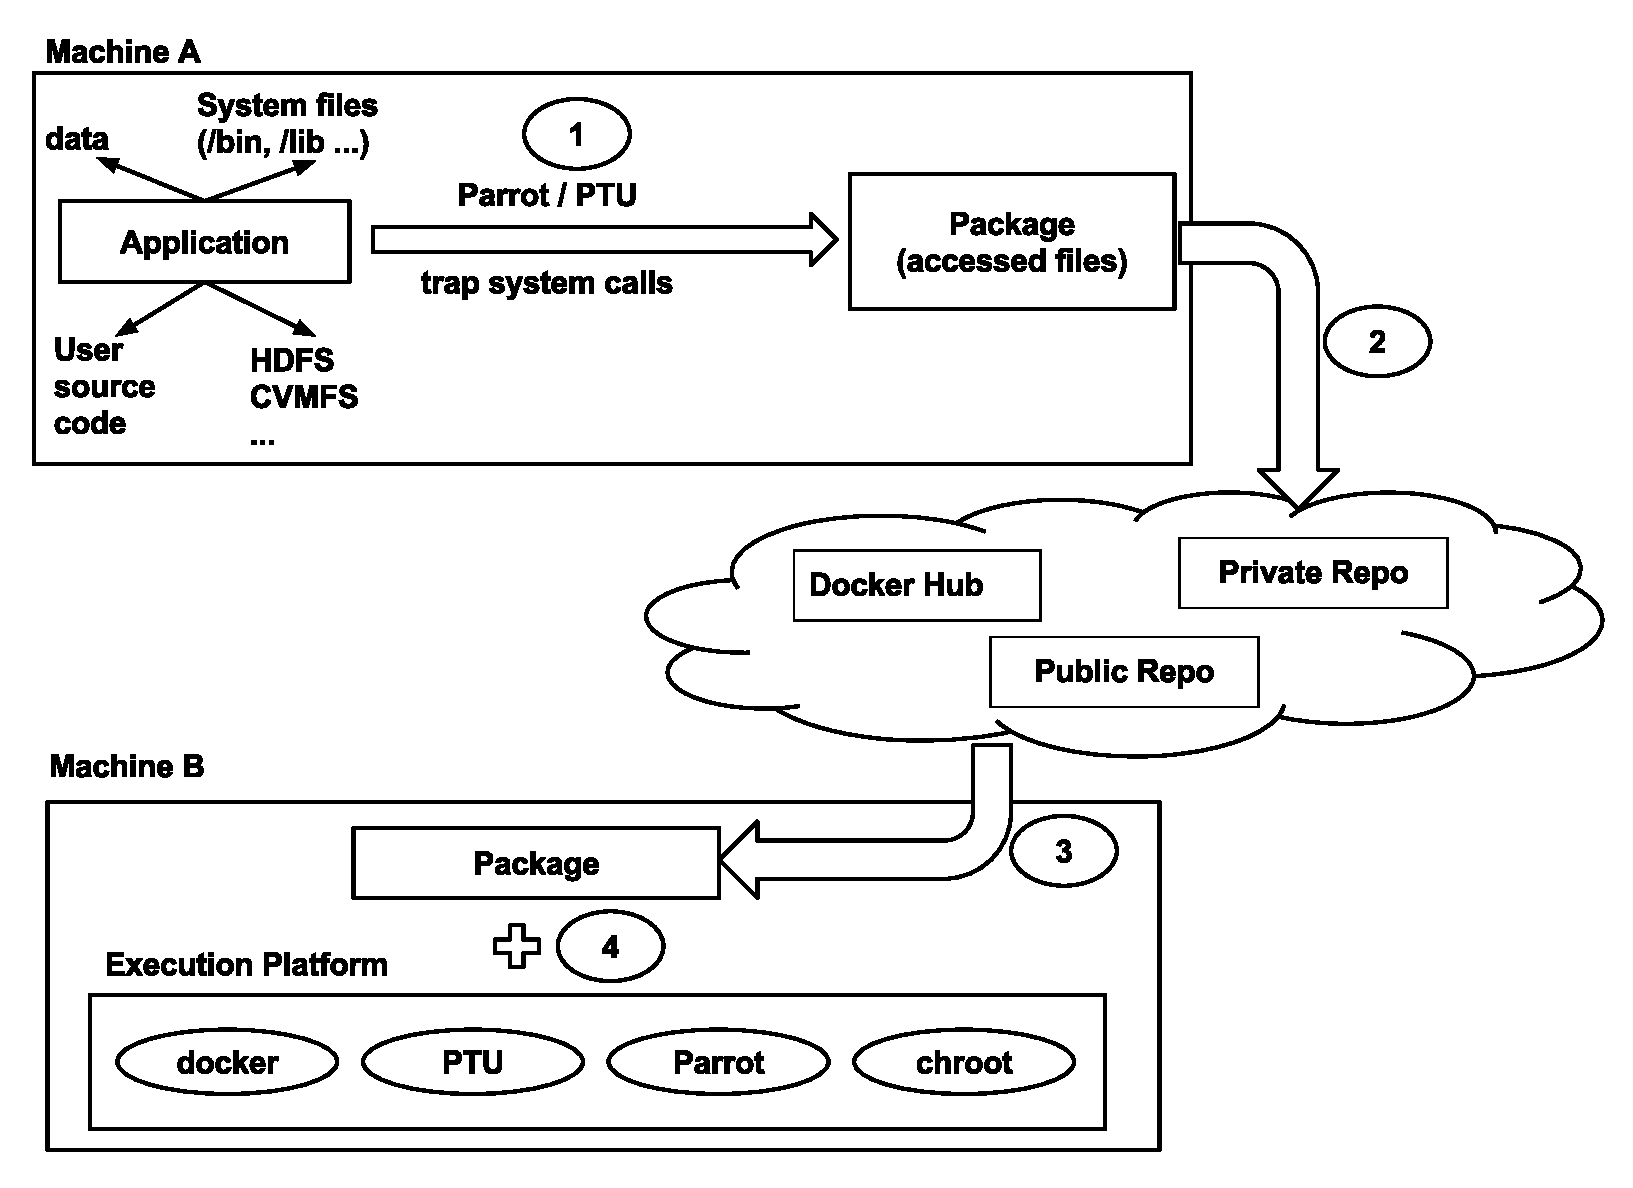
\includegraphics[width=.8\textwidth]{preservation_framework.eps}
\caption{Preservation Framework}
\label{fig: preservation_framework}
\end{figure*}

%\section{Measuring Dependencies}
%We have developed a prototype tool to assist in the measurement and preservation
%of implicit dependencies for complex applications.
%We use Parrot~\cite{thain2005parrot} to explicitly record all
%of the files accessed by our example application, allowing us to observe how
%much of each external dependencies is used, and what local resources are implicitly used.
%Using this information, we create a \emph{reduced package} which contains
%only the files actually used by the application.
%
%Parrot is a virtual filesystem access tool which has been used to attach
%existing programs to a variety of remote I/O systems, such as HTTP, FTP, and CVMFS.
%It works by trapping an application's system calls through the Linux {\tt ptrace} debugging
%interface, and then replacing them with the desired I/O operations.  Parrot is already used
%in the high energy physics community with applications like TauRoast specifically to 
%provide access to the CMSSW software distribution via the CVMFS distributed file system.
%We made small modifications to Parrot to record a \emph{namelist} which lists all 
%of the files that an application actually accesses.
%
%Figure~\ref{fig:workflow-parrot} illustrates the measurement process.
%The starting point of this toolkit is one successful execution of the application on the native machine.
%First, we execute the actual data analysis script under Parrot to generate the namelist.
%Then, using the namelist, we generate a package containing all the necessary data
%and software for one analysis program. When another
%researcher wants to repeat the program, he only needs to obtain the package and
%execute the actual analysis program inside the package. 
%
%For one execution of \emph{TauRoast}, the generated namelist includes 132,047 accessed filenames,
%along with the system calls used to access the file, such as {\tt open}, {\tt stat}, {\tt read}, etc.
%With duplicate filenames removed, the list is reduced to 67,168 files.
%Many of those entries do not exist, because they reflect attempts
%by the application to search for programs and libraries in multiple places.
%Only 22,068 entries reflect existing files or directories.
%
%The packaging tool iterates over each item of the filename list, determines the process
%mode and replication degree according to the file type (common files,
%directories, symbolic links) and the system call type, generates one package
%containing the dependencies, and summarizes the contents of the package
%as shown in Table~\ref{table:package-info}.  To the extent possible,
%the filesystem structure of the original environment is preserved.
%
%We considered several approaches to constructing the package.
%In a {\bf shallow copy}, we only copied the individual files in the namelist,
%creating only parent directories for each.  Where a directory was listed,
%we created the directory and populated it with empty files as placeholders
%to facilitate a directory listing.  In a {\bf medium copy}, we copied the
%individual files as before.  Where a directory was listed, we created
%the directories and copied the contents of the files in that directory,
%one level deep.  A {\bf deep copy} would duplicate all directories recursively,
%but this would have resulted in TB-sized packages, so we did not consider
%it further.
%
%Parrot is required to re-run the packaged artifact, in order to force
%the packaged files to appear to exist in their original locations.
%To this end, the packaging tool creates a \emph{file map} which maps
%the logical names of the files to their current physical locations, as shown in Table~\ref{table:map-file}.
%Parrot reads the file map and redirects system calls at run-time to achieve the desired effect.
%As the example suggests, special device files such as {\tt /proc} and {\tt /dev}
%are not incorporated into the package but are instead accessed natively.
%
%\begin{table}
%    \centering
%    \begin{tabular}{ll}
%    \hline
%    \bf Path used in Program & \bf Actual Location \\ \hline
%    {\tt /} & {\tt /tmp/package-hep} \\ \hline
%    {\tt /tmp/package-hep} & {\tt /tmp/package-hep} \\ \hline
%    {\tt /dev} & {\tt /dev} \\ \hline
%    {\tt ...} & {\tt ...}\\ \hline
%    \end{tabular}
%    \caption{Structure of Map File}
%    \label{table:map-file}
%\end{table}
%
%\begin{table}
%    \centering
%    \begin{tabular}{rrr}
%\hline
%                    & \bf Shallow Copy & \bf Medium Copy\\
%\hline
%    Whole Files    & 1632         & 15642\\ 
%\hline
%    Empty Files    & 14273        & 263\\
%\hline
%    Directories    & 1549         & 1549\\ 
%\hline
%    Symbolic Links & 4614         & 4614 \\
%\hline
%    \bf Total Size & \bf 21GB     & \bf 28GB \\ 
%\hline
%    \end{tabular}
%    \caption{Package Information}
%    \label{table:package-info}
%\end{table}

%\subsection{Tracking of Network Dependencies}
%
%\begin{figure}
%\centering
%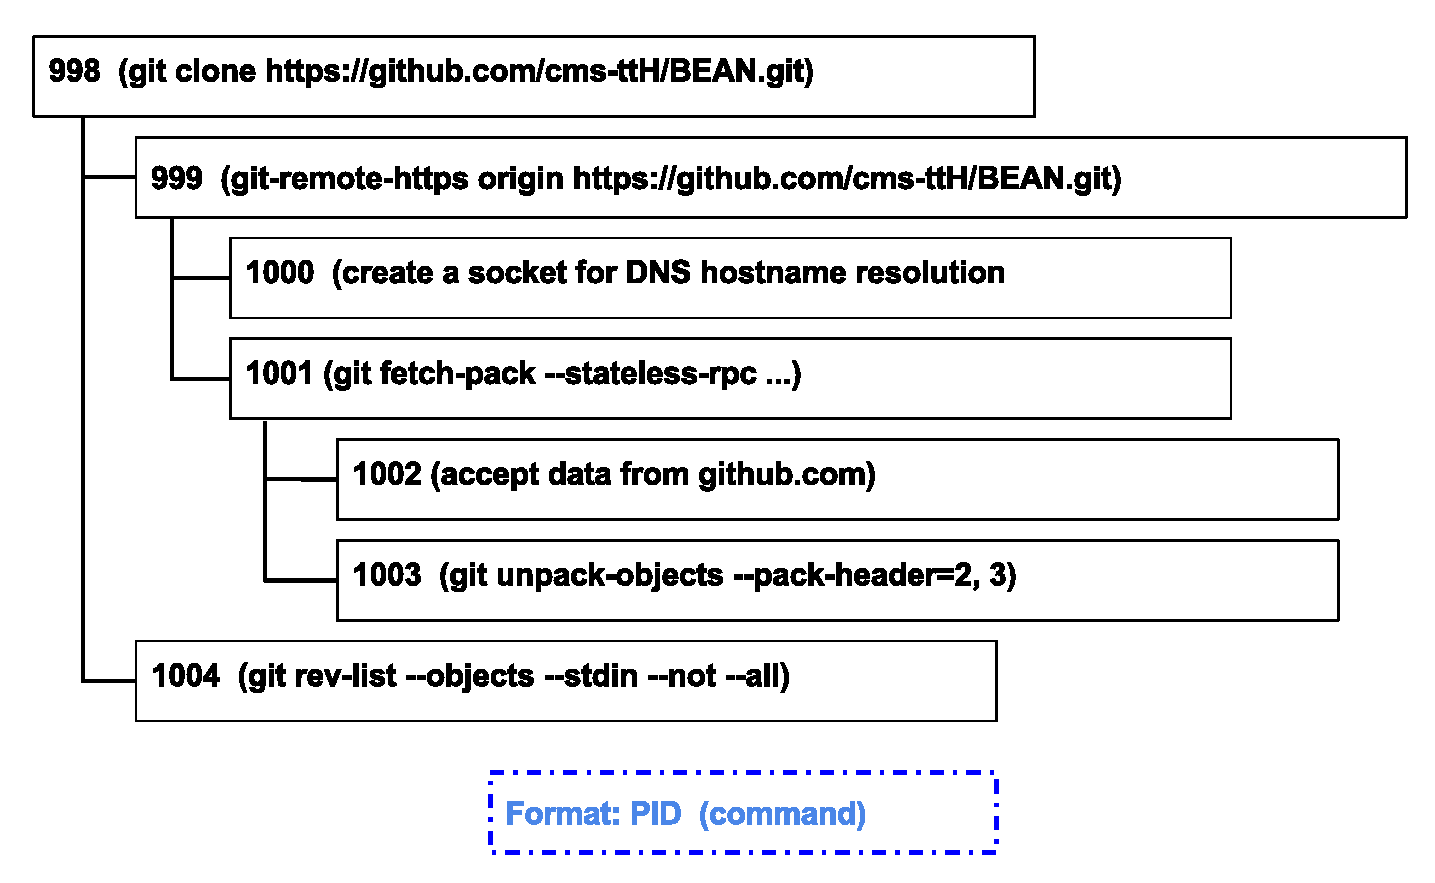
\includegraphics[width=.6\textwidth]{git-syscall.eps}
%\caption{Exec Syscalls of a git command}
%\label{fig:git-syscall}
%\end{figure}
%
%\begin{figure}
%\centering
%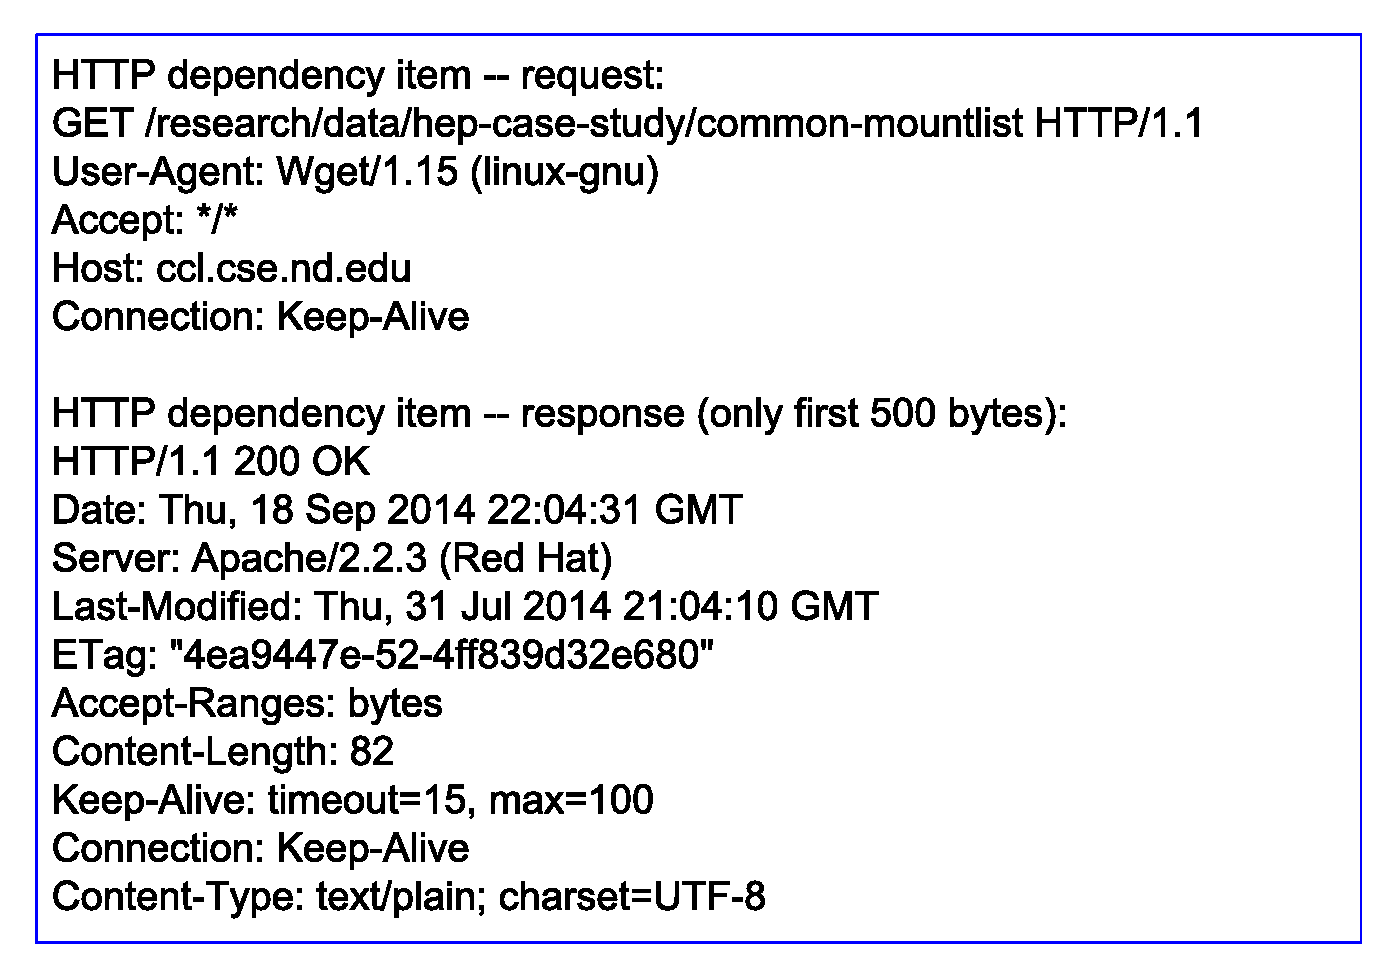
\includegraphics[width=.6\textwidth]{http_packet.eps}
%\caption{HTTP Request and Response}
%\label{fig:http_packet}
%\end{figure}
%
%\begin{figure}
%\centering
%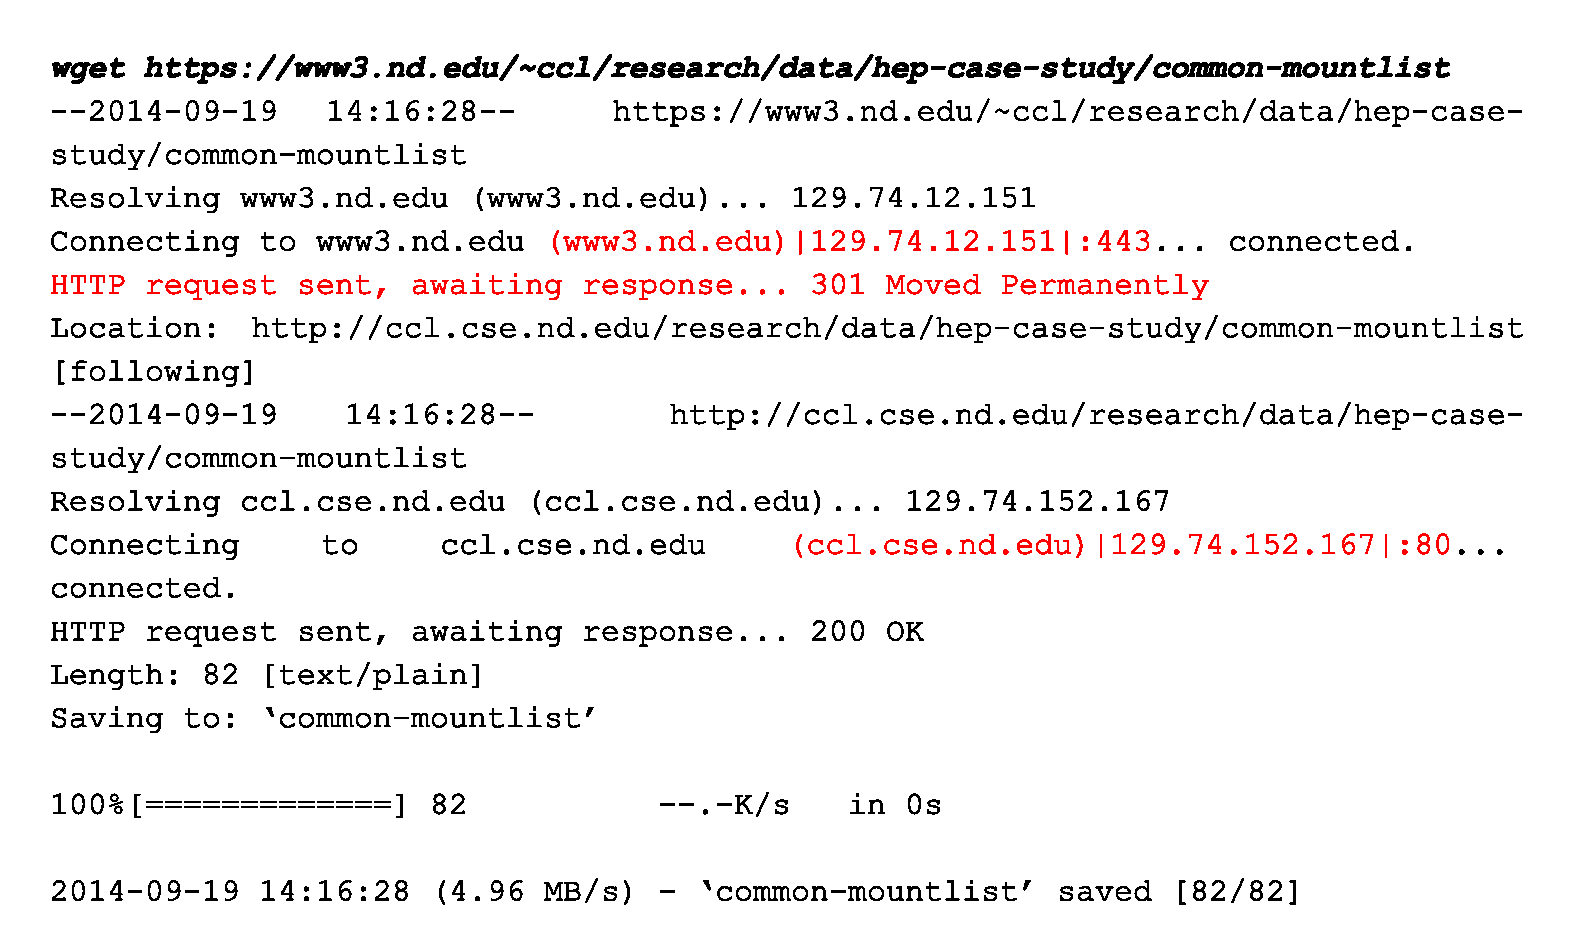
\includegraphics[width=.6\textwidth]{url_redirection.eps}
%\caption{An Example of URL Redirection}
%\label{fig:url_redirection}
%\end{figure}
%
%All the dependencies of one program can be divided into three categories: local file system (e.g., /usr, /lib and /lib64), remote file systems which can be mounted as local directories (e.g., /cvmfs and /hdfs), and other remote network dependencies (e.g. http, https and ssh).
%Through utilizing ptrace to trap each file-relevant system call used by a program, the first two categories of dependencies can be collected. 
%Motivation of tracking network dependencies: Linkrot is a common and great threat to the preservation of scientific applications. A URL which works normally today may be unavailable permanently. A method which can help the scientists figure out all the network dependencies of their applications provides the chance to evaluate the stability of each network dependencies and preserve the unstable network resources before linkrot happens.
%One direct solution to track the third category of dependencies is to utilize ptrace to check each exec system call used by a program and record each network-relevant executable and its parameters. However, an executable may create one or more child processes to finish some tasks, and a child process may create their own children processes. Figure~\ref{fig:git-syscall} shows all the processes created by a git command. A process with PID 998 is created to clone a remote git repository into local machine, which totally has 6 child processes. Moreover, a network-relevant executable name collection is necessary to identify network dependencies. The diversity of network-relevant executables and the large process tree generated for a network executable make this solution infeasible.
%
%Another solution to track network dependencies is to track the network sockets. The user process communicates with the network protocol stacks in the kernel through the network socket layer user interface on Linux. From the process tree shown in the above figure, the process with PID 1000 responds to create a socket, connect to a DNS server, send a DNS request packet to the DNS server and receive a DNS response packet from the DNS server. The information gained from the network socket tracking can be divided into three categories.
%\begin{itemize}
%\item The information of network sockets used to communicate with remote network dependences (through socket and connect system calls) can be used to figure out the port number, service name (such as, http, https, and ssh), socket type (stream and datagram),  and the domain type (inet and inet6). 
%\item The contents of DNS packets can be used to figure out the hostname and IP address of each remote network dependency. 
%\item As for applications based on http protocol, all the http requests and responses can be seen, as shown in Figure~\ref{fig:http_packet}. However, as for applications based on https and ssh which encrypt network data using TLS/SSL, tracking network data on the socket level can only see the encrypted data. 
%\end{itemize}
%
%The results of tracking network sockets used by a program involves two categories of network resource redirections, dns-level hostname redirection and website-level url redirection. 
%\begin{itemize}
%\item dns-level hostname redirection: Each DNS packet includes five parts, header, question, answer, authority, and additional. A DNS response packet with the type CNAME has multiple answers. For example, the DNS response packet which tries to resolve {\tt www3.nd.edu} includes two answers. The first answer provides an alias of {\tt www3.nd.edu}, {\tt www-vip.cc.nd.edu}, and the second answer maps the alias to the IP address. 
%{\tt www3.nd.edu} CNAME {\tt www-vip.cc.nd.edu}
%{\tt www-vip.cc.nd.edu} A {\tt 129.74.12.151}
%The CNAME-type DNS packets leave us a question, among the hostname used by the user, the alias(es), the IP address, what should we preserve?
%\item website-level url redirection: Website-level url redirection happens when a website updates its location and still want their old users access their resources using the old url. Figure~\ref{fig:url_redirection} illustrates the url redirection between {\tt \url{www3.nd.edu/~ccl}} and {\tt ccl.cse.nd.edu}. Except for the difference of hostnames, the application layer protocols used by the old-version website and the new-version website is also different: the old website provides services through the https protocol, while the new website provides services through the http protocol. 
%\end{itemize}
%
%The usage of https protocol makes detecting of website-level url redirections through tracking system calls more difficulty and even impossible. All the application data will be encrypted at presentation layer through the TLS/SSL protocol, which is initialized at the session layer and works at the presentation layer.


\section{Evaluation}

We evaluated the correctness of the reduced package and the overhead of generating the package.
To do this, the application was repeated with the help of \emph{Original Script} (as shown in Figure~\ref{fig:version-evolution}) on the original machine. 
Then one \emph{reduced package} was generated and verified with the help of Parrot on the original machine.

Then, two different virtual machines (VM) - one VM from the Notre Dame Cloud Platform based on KVM and one VM from the Amazon EC2 Platform based on Xen, were employed to further verify the correctness of the reduced package.

We first repeated the example from scratch using the Script translated from the original email on the original machine and counted the time consumption and data size. 
Then based on the successful execution of Original Script, we evaluated Reduced Package - one package containing necessary dependencies is generated, and then the time consumption and data size is analyzed. 

To measure time consumption, we counted the time used to obtain remote software dependencies, build the environment, and analyze the dataset. We also counted the time used to obtain the namelist and to generate the package. To measure data size, we can easily figure out the size of each data and code source inside the package under Reduced Package.
Original Script does not support mining of implicit dependencies. As for remote sources, we can figure out the named size through the analysis script. However, it is hard to figure out the named size of each local source. 
Instead, we only knew that total size of each file system is very large.

Table~\ref{table:time-2nd3rd} shows the execution time comparison between
Original Script and Reduced Package.
Reduced Package is faster than Original Script, because all the software copied into the package has been compiled and the Software Acquisition stage is not necessary.
and all the environment building only takes 4 seconds,
We were surprised that Reduced Package even reduces the actual analysis time. 
The reason for this is that data is obtained through accessing HDFS in Original Script, but is copied into the package in Reduced Package. This localization of experimental data speeds up the data analysis process, resulting the actual analysis time reducing from 20 minutes to 13 minutes.

\begin{table}
    \centering
    \begin{tabular}{lrr}
    \hline
    \bf Task Category & \bf Original Script & \bf Reduced Package \\ \hline
    Obtain Namelist & N/A & 28min 28s \\ \hline
    Generate Package & N/A & 85min 51s \\ \hline
    Software Acquisition & 8min 11s & N/A \\ \hline
    Environment Build & 5min 49s  & 4s \\ \hline
    Analysis Code & 20min 31s & 13min 04s \\ \hline
    \end{tabular}
    \caption{Execution Time Comparison between Original Script and Reduced Package}
    \label{table:time-2nd3rd}
\end{table}    

Table~\ref{table:time-2nd3rd} also illustrates the time used to
obtain the namelist and to generate the package. 
The time used for these two steps is longer than the execution time,
because each filename of the list, together with its system call type, needs to be checked, and the structure of each directory item must be maintained.
However, 
this is only done once.
Once the package is
generated, many users can directly obtain the package and repeat the application 
separately. 

Table~\ref{table:size-original-real} on page 2 illustrates the total size, named size in the example and actually used size of each remote source (the first 4 items) and local source (the remaining 5 items).
The third column corresponds to the data size of Reduced Package and can be easily figured out, because all the necessary data has been copied into the package.
Original Script does not support measuring implicit dependencies. As for remote sources, we can figure out the named size through the analysis script. However, it is hard to figure out the named size of each local source. 
Instead, we only knew that total size of each file system is very large.

\begin{table}
	\centering
	    \begin{tabular}{llrrr}
	        \hline
	        \bf Name & \bf Location & \bf Total & \bf Named & \bf Used \\ 
	        \hline
	        CMSSW code     & CVS & 88.1GB & 448.3MB & 6.3MB\\ \hline
	        Tau source       & Git & 73.7MB & 73.7MB & 6.7MB \\ \hline
	        PyYAML binaries    & HTTP & 52MB & 52MB & 0KB \\ \hline
	        .h file       & HTTP& 41KB & 41KB & 0KB \\ \hline \hline
	        Ntuples data    & HDFS& 11.6TB & N/A& 20GB \\ \hline
	        Configuration & CVMFS & 7.4GB & N/A & 103MB \\ \hline
	        Linux commands & localFS & 110GB &  N/A & 68.4MB \\ \hline     
	        HOME dir& AFS &12GB & N/A & 32MB\\ \hline
	        Misc commands & PanFS & 155TB & N/A  & 1.6MB \\ \hline
	        Total      &    & 166.8TB            & N/A & 21GB \\ \hline
	    \end{tabular}
	    \caption{Data and Code Used by Tau Roast}
	    \label{table:size-original-real}
\end{table}
%	\begin{tablenotes}
%	      \small
%	      \item The first column illustrates the total size of each data and software source; 
%	            the second column illustrates the size of the named files from each source;
%	            the third column illustrates the size of actually used data from each source.
%	            N/A denotes it is hard to figure out the named size of implicit dependencies directly.        
%	    \end{tablenotes}
	    
To further verify the correctness of Reduced Package on other machines, two different machines are employed -
one virtual
machine~\cite{goldberg1974survey} from the Notre Dame Cloud Platform based on KVM sharing the same kernel version with the original machine,
and one virtual machine from  the Amazon EC2~\cite{amazon2010amazon} Platform based on Xen.

Table~\ref{table:config-vm} illustrates the configuration of 
each machine and the execution time of the application on each machine.
All the machines adopt the x86\_64 hardware platform and Linux kernel.
Both of the two VMs repeated the application with the help of the package generated on the original machine successfully.
The execution time on one machine greatly depends on its hardware configuration.

\begin{table}
    \centering
    \begin{tabular}{lrrrr}
    \hline
    \bf Machine Type & \bf Distro Version & \bf CPU Cores & \bf Mem (GB) & \bf Execution Time \\ \hline 
    Original Machine &  Red Hat 5.10 & 64 & 125 & 13min 04s\\  \hline
    KVM (Notre Dame) & CentOS 5.10 & 4 & 2 & 21min 38s\\ \hline
    Xen (EC2) & Red Hat 5.9 & 16 & 60.5 & 13min 30s\\ \hline
    \end{tabular}
    \caption{Evaluation of Different Machines}
    \label{table:config-vm}
\end{table}

In summary, we demonstrate that the application can be repeated with the help of the reduced package on one different machine with the required hardware architecture and OS kernel version.
%*****hmeng-doubt:Another reason for the packaging utility is that not all the data and software generated by the second version script is used during the the actual data analysis. The packaging utility can help us find out the optimal subset of data and software involved in one actual data analysis. 
%*****hmeng-doubt: this point is not the motivation. but one achievement comes together. out of imagination.


%\begin{figure}
\centering
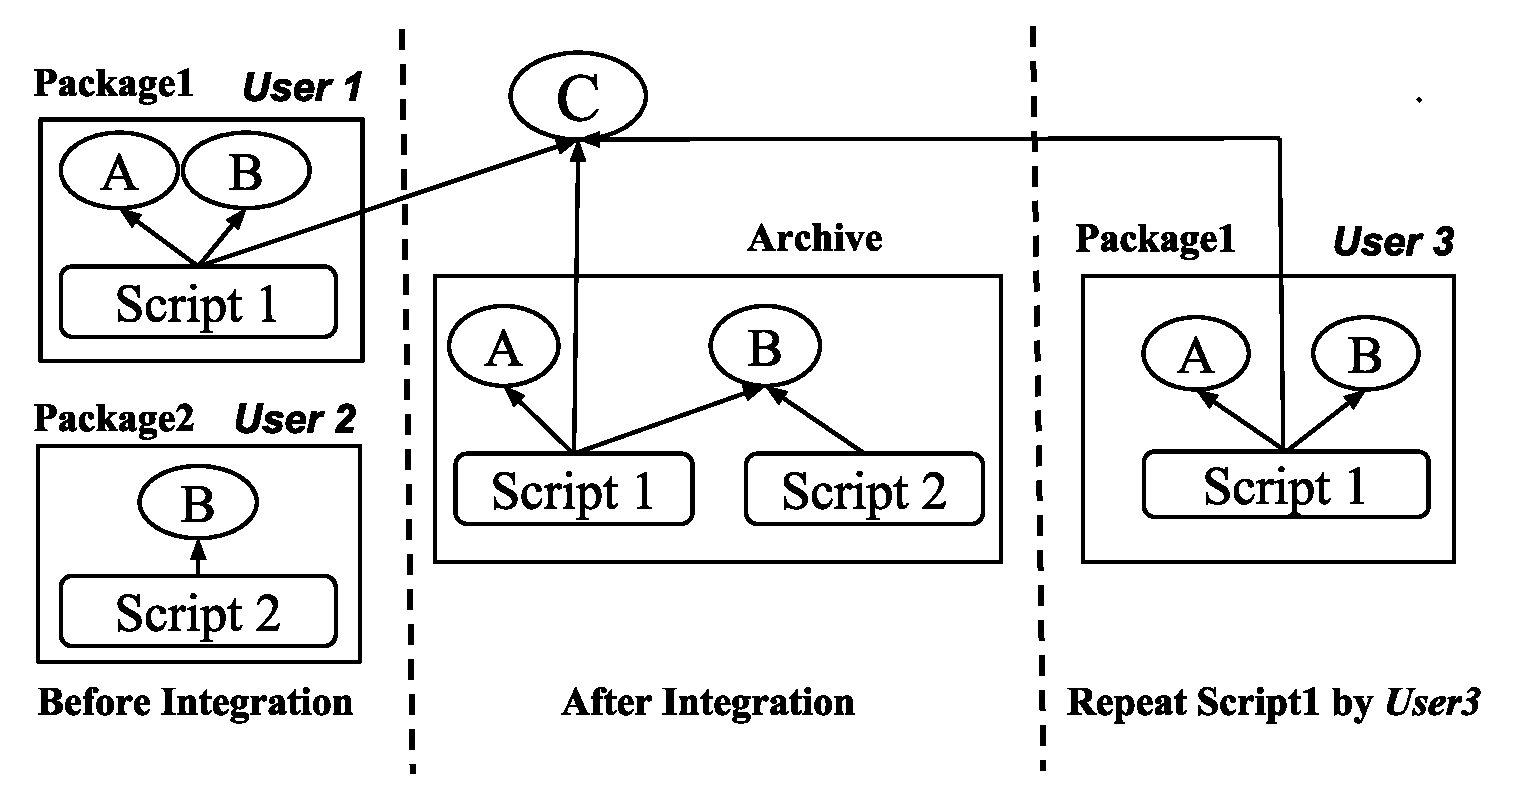
\includegraphics[width=.6\textwidth]{preservation-integration.eps}
\caption{Preserving Multiple Artifacts}
\label{fig:Preservation integration}
\end{figure}

\section{Open Problems}

Figure~\ref{fig:Preservation integration} shows the rough information
architecture of the archive that we imagine for complex
scientific software like TauRoast.
Each artifact to be preserved is a package that consists of a top-level
script to invoke the software, a dependency map, and the dependencies
themselves, which may be external to the original program.  The artifacts
are then ingested into the archive, where shared dependencies are stored
only once.  In cases where an artifact has a dependency on a trusted
(or very large) remote archive, the dependency may simply be tracked
. A researcher that wishes to reproduce a given
result need only refer to the unique identifier of the artifact, and will
be able to automatically extract all of the dependent components of
that artifact.

For example, in Figure~\ref{fig:Preservation integration} Script 1 depends on items A, B, and C.  Items A and B are ingested into the archive, where B is shared with Script 2.  Item C is stored in another trustworthy repository and is tracked rather than ingested.  When Script 1 is exported from the repository, items A and B are exported along with it, while C can be copied or remain remote, according to the end user's choice.

As simple as that picture appears, there are a number of problems that must be solved to get there:

{\bf Measure the Mess or Force Cleanliness?}  Two radically different approaches to dependency tracking are possible.  The first is to allow end users complete freedom to construct their environment as desired, then \emph{measure} what items were actually used.  As we have shown, this is possible, but has significant overheads and does not fully preserve the structure or intent of the end user.   The second approach is to \emph{force} users to work in a clean environment in which no resource can be used until a proper dependency has been declared.  This ensures that all dependencies are known in advance (and made explicit to the end user) but places a variety of restrictions on the user's daily work, and may prevent creative approaches that do not fit within the curator's view of how programs should be structured.  Whether end users will accept the inconvenience of forced cleanliness for the benefits of reproducibility can only be discovered through experiment.

{\bf Granularity of Dependencies.}  Dependencies could be handled
at many different levels of granularity.  In this work, we have shown
how they can be handled at the level of entire repositories or individual files.
Other possible choices might include intermediate-sized software packages
(like RPM) or in the case of experimental data, even portions of individual large files.  Clearly, a larger granularity will result in 
simpler dependency maps, and more wasted space; smaller granularity results
in complex dependency maps and less wasted space.  A hybrid solution may
be able to combine both by storing large granularity dependencies, but
selecting sub-items out of objects when efficiency demands it.

{\bf Scope of Reuse.}  We have presented the data preservation
problem as primarily one of accurate reproduction: if a result depends
on running program X, we must be able to run exactly X again.  However,
the goal of scientific reproducibility is rarely limited to running
\emph{precisely} what a predecessor did. Often, the objective is to
change a parameter or a data input in order to see how the result is affected.
To that end, the preservation system must capture enough of the surrounding
material to permit modifications to succeed.  From this perspective,
a larger granularity of preservation is desirable.  A better understanding of
how end users will consume preserved software will help to shape how
software is preserved in the first place.

{\bf Dependency Detection.}  If we allow users to work in uncontrolled
environments, then we must have better methods for understanding the dependencies  of existing programs.  At first, we relied on an expert reader to examine
the user's script and extract the dependencies.  This is clearly
not a scalable approach.  We then demonstrated an automated method of observing
what individual files are accessed by a program. However, this does
not cover all types of dependencies, particularly those that are networked.
More sophisticated observation techniques could infer higher-level information,
such as the RPM package names of the files accessed, the URLs of remote
repositories named throughout the program, or even the addresses and names of networked dependencies like databases and filesystems.

{\bf Source, Binary, or Both?}  A science archive might choose to retain
the source code of an artifact or the binary code that can actually run in a given environment.
While conventional wisdom suggests that access to source code is critical for the long term
survival and evolution of a piece of software, it also requires the maintenance of an enormous
amount of supporting software in the form of compilers, linkers, and supporting libraries for
the target platform.  Rebuilding all of these for every invocation of an artifact is
likely to have excessive cost.  We suggest that a realistic repository will have to
maintain \emph{both}: the source describes the ultimate meaning of the code, but
the binary is an important performance cache, a backup if the compiler toolchain should
fail to be preserved, and a checksum to ensure that a source artifact was rebuilt correctly.


\section{Related Work}

%Generally, there are three approaches to preserve a software environment:
%hardware preservation, migration and emulation.  Hardware
%preservation preserves the original software and its original operating
%environment. 
%Software migration technique~\cite{cifuentes1996binary,mancl2001refactoring} is used to facilitate running software on new machines.
%However, migration often involves the re-compiling and re-configuring
%the source code to accommodate a new hardware platform and software environment.
%Emulation recreates the original software and hardware environment by
%programming future platforms and OSs. Virtual machine is one common way to implement this. According to the usage and degree of emulation of the real
%machine, virtual machine can be divided into system virtual machine and process
%virtual machine. The working and design principles and
%performance evaluation of system virtual machine were illustrated in~\cite{goldberg1974survey, smith2005architecture}. 
%Further, the functionality of system VM to support different guest operating systems was illustrated in~\cite{barham2003xen,kivity2007kvm,rosenblum1999vmware}.
%%F. Esquembre~\cite{esquembre2004easy} illustrated how JVM, one process virtual machine, can expedite the creation of
%%scientific simulations in Java. 
%The pros and cons of these three approaches were discussed in~\cite{matthews2009towards,phelps2005no,hong2010software}.

The capture and preserve environments were treated as one entity in~\cite{matthews2009towards,phelps2005no,hong2010software}. 
However, frequently changing experiment software makes the maintenance of the captured experimental environment very complex. 
CernVM~\cite{buncic2010cernvm} treated them as two different categories. 
The capturing of computing environment is implemented within CernVM, and the preservation of software environment is based on a CernVM filesystem(CVMFS) specifically designed for efficient software distribution.
In fact CVMFS~\cite{buncic2010cernvm} published pre-built and configured experiment software releases to avoid the time-consuming software building procedure, i.e, it did not 
preserve software in source code format as emphasized in~\cite{zabolitzky2002preserving,castagne2013consider}. 
However, as we show a simple VMI of binaries can also be too big in size for distribution, and the preservation itself needs to include a documentation stage and a distribution stage. 
We have described capture tools that include software code when available to be included in the package. 

%Current mechanisms of preserving scientific experiments assume that all the data and software mentioned in the experiments are necessary for the reproduction of the experiments. 
%However, this is not always the case. In some cases, the original author may leave additional code referring to irrelative data and software in the application or the application may require additional 
%data and software for reproducibility. 

%One mechanism, which can figure out the absolutely relevant data and software of one experiment, is important for both the preservation and reproduction of scientific experiments.

Attempts from different perspectives to facilitate the reproduction of scientific experiments utilizing a preserved software library have been made. 
The software distribution mechanism over network was discussed in~\cite{compostella2010cdf, blomer2011cernvm}.
J. R. Rice et al.~\cite{rice1996scientific} describe a distribution hub through the integration of user interface, scientific software libraries, knowledge base into problem-solving environment.
S. R. Kohn et al.~\cite{kohn2001divorcing} tried to enable the creation and distribution of language-independent software library by addressing language interoperability.
a scalable, distributed and dynamic workflow system for digitization processes was proposed in~\cite{schoneberg2013scalable}.
A distributed archival network was designed in~\cite{subotic2013distributed} to facilitate process-oriented automatic long-term digital preservation.
M. Agosti et al.~\cite{agosti2012envisage} aimed to help non-domain users to utilize the digital archive system developed for domain experts.

%B. Matthews et al.~\cite{matthews2008significant} introduced one conceptual framework for software preservation from several case studies of software preservation.
%One tool to capture software preservation properties within a software environment was designed in~\cite{matthews2010framework} through a series of case studies conducted to evaluate the software preservation framework.
%L. R. Johnston et al.~\cite{johnston2014workflow} proposed one overall data curation workflow for 3-5 case studies of preserving research data.
%Two case studies~\cite{borgman2012data} were conducted to figure out the properties of data to be reused in the future.




%Generally, there are three approaches to preserve a software environment:
%hardware preservation, migration and emulation.  Hardware
%preservation preserves the original software and its original operating
%environment. 
%Software migration technique~\cite{cifuentes1996binary,mancl2001refactoring} is used to facilitate running software on new machines.
%However, migration often involves the re-compiling and re-configuring
%the source code to accommodate a new hardware platform and software environment.
%Emulation recreates the original software and hardware environment by
%programming future platforms and OSs. Virtual machine is one common way to implement this. According to the usage and degree of emulation of the real
%machine, virtual machine can be divided into system virtual machine and process
%virtual machine. The working and design principles and
%performance evaluation of system virtual machine were illustrated in~\cite{goldberg1974survey, smith2005architecture}. 
%Further, the functionality of system VM to support different guest operating systems was illustrated in~\cite{barham2003xen,kivity2007kvm,rosenblum1999vmware}.
%%F. Esquembre~\cite{esquembre2004easy} illustrated how JVM, one process virtual machine, can expedite the creation of
%%scientific simulations in Java. 
%The pros and cons of these three approaches were discussed in~\cite{matthews2009towards,phelps2005no,hong2010software}.
%
%The preservation of computing environment and software environment was treated as one entirety in~\cite{matthews2009towards,phelps2005no,hong2010software}. 
%However, frequently changing experiment software makes the maintenance of the preserved experimental environment very complex. 
%CernVM~\cite{buncic2010cernvm} treated them as two different categories. 
%The preservation of computing environment is implemented with CernVM, and the preservation of software environment is based on a CernVM filesystem(CVMFS) specifically designed for efficient software distribution.
%In our work, we have distinguished between capture and preserve phases but extended to include automated mechanisms. 
%
%The importance of preserving software in source code format was emphasized in~\cite{zabolitzky2002preserving,castagne2013consider}. 
%However, CVMFS~\cite{buncic2010cernvm} published pre-built and configured experiment software releases to avoid the time-consuming software building procedure. 
%
%Attempts from different perspectives to facilitate the reproduction of scientific experiments utilizing a preserved software library have been made. 
%The software distribution mechanism over network was discussed in~\cite{compostella2010cdf, blomer2011cernvm}.
%J. R. Rice et al.~\cite{rice1996scientific} made the reproduction process easier through the integration of user interface, scientific software libraries, knowledge base into problem-solving environment.
%S. R. Kohn et al.~\cite{kohn2001divorcing} tried to enable the creation and distribution of language-independent software library by addressing language interoperability.
%a scalable, distributed and dynamic workflow system for digitization processes was proposed in~\cite{schoneberg2013scalable}.
%A distributed archival network was designed in~\cite{subotic2013distributed} to facilitate process-oriented automatic long-term digital preservation.
%M. Agosti et al.~\cite{agosti2012envisage} aimed to help non-domain users to utilize the digital archive system developed for domain experts.
%
%Current mechanisms of preserving scientific experiments assume that all the data and software mentioned in the experiments are necessary for the reproduction of the experiments. However, this is not always right. In some cases, the original author may leave additional code referring to irrelative data and software in the program. One mechanism, which can figure out the absolutely relevant data and software of one experiment, is important for both the preservation and reproduction of scientific experiments.
%
%B. Matthews et al.~\cite{matthews2008significant} introduced one conceptual framework for software preservation from several case studies of software preservation.
%One tool to capture software preservation properties within a software environment was designed in~\cite{matthews2010framework} through a series of case studies conducted to evaluate the software preservation framework.
%L. R. Johnston et al.~\cite{johnston2014workflow} proposed one overall data curation workflow for 3-5 case studies of preserving research data.
%Two case studies~\cite{borgman2012data} were conducted to figure out the properties of data to be reused in the future.
%

%\section{Postscript}

We began this work in late 2013, generating a reduced package for \emph{TauRoast} based
on the configuration of a standard machine at Notre Dame at the time.  In the course
of writing this paper in spring 2014, almost everything about the computing environment
changed: the operating system was upgraded, a new version of CMSSW was released, and
our local HEP users switched from using CVS to CVMFS for accessing CMSSW.
The original script provided by the author failed to run on the same machine.
But, the reduced package we created three months earlier in the old environment
worked just fine on the new machine.



\section*{Acknowledgments}

This work was supported in part by National Science Foundation grants PHY-1247316 (DASPOS), 
OCI-1148330 (SI2), PHY-1312842, ICER-1440327, SES-0951576 (RDCEP), and ICER-1343816 (UChicago subcontract).
The University of Notre Dame Center for Research Computing scientists and engineers provided critical technical assistance throughout this research effort.
The Open Science Grid at the University of Chicago provided critical technical assistance throughout this research effort.

\bibliographystyle{plain}
\bibliography{cclpapers,this}

\end{document}

\if 0
Section 2: Overview of Application
    CMS/LHC introduction.
    Data sources and reduction of size.
    Code sources and reduction of size.
    Prose observations about the script.
        Uses multiple repos that change over time, with varying level of stability.
        Low selectivity from the larger repos
        Significant initialization time to collect everything.
        Incidental infrastructure tools versus essential objects.
        Some dependencies were surprising.
    Figure: Diagram of app with both code and data sources.
    Table: Show all code and data sources and size within one table.

Section 3: Preservation Strategies
    Figure: Show app in four stages:
        Single email.
        Script with embedded references to dependencies.
        Script with map file that refers to external dependencies.
        Script with map file that refers to preserved dependencies.

    Transform to more suitable format that expresses dependencies.

    Incorporate into archive, saving deps and map file.

    But, how to get the dependencies?

    Three strategies:
        Original - Unmodified application run in original environment.
        Coarse-Grained - Capture deps at large granularity -- whole filesystems and repositories.
        Fine-Grained - Capture deps at a fine granularity -- individual files actually used.

    Coarse-Grained Method (Copy Repositories)
        First, determine dependencies
        Express app as script + map file
        Packaging tool downloads deps, rewrites map file.
        To run packaged application, obtain map, download

    Fine-Trained Toolkit (Parrot)
        Tool to detect dependencies (Parrot)
        Express app as script + map file
        Packaging tool downloads deps, rewrites map file.
        To run package application, run again with Parrot.

Section 4: Evaluation

    Table: Time and size of preserving using each of the two techniques.

    Explain why the techniques show different performance.

    Is one technique more effective than the other?  Why?
\fi

